Die paarweise Kollisionserkennung bezieht sich auf die Kollision von konkret zwei 3D-Modellen. In diesem Schritt ist die Genauigkeit der Kollision bei steigender Modellkomplexität im Fokus.
Ziel ist es die Diskrepanzen zwischen der grafischen Anzeige von Modellen und der physikalischen Simulation zu deckeln.
\subsection{Input}
Aus dem vorhergehenden Schritt der Kollisionspaarermittlung werden für den Schritt der paarweisen Kollisionserkennung bis zu  $|OBJ|^2$ Objektpaare $C_{guess}\subseteq OBJ^2$ erhalten, für die eine Kollisionsvermutung während eines Ticks gilt. Man geht weiter davon aus, dass die Menge der tatsächlichen Kollisionen $C_{definitive}\subseteq OBJ^2$ in der Menge der vermuteten Kollisionspaare  vollständig enthalten ist $C_{definitive}\subseteq C_{guess}$, d.h. keine tatsächlichen Kollisionspaare im Paarermittlungsprozess verloren gehen. 

\subsection{Output}
Es ist eine Aufgabe dieses Schritts, die Reduzierung von $C_{guess}$ auf $C_{defintive}$ zu vollenden.\\
Eine zweite Aufgabe ist die Ermittlung von Informationen über den Hergang der Kollisionen der Paare in $C_{defintive}$.
Im Abschnitt~\ref{sec:usages} werden einige Verwendungszwecke der Kollisionsermittlung aufgelistet. 
Elemente der Aufzählung haben unterschiedliche Anforderungen hinsichtlich benötigter Information über den Kollisionsvorgang um realisiert werden zu können.

\begin{enumerate}
	\item Schnitt\\
		Die Frage ob Objekte $o_0,o_1 \in OBJ$ sich an einem konkreten Zeitpunkt während eines Ticks $t\in \Upsilon_{\delta i}$ schneiden/gegenseitig enthalten. $K_{o_0, t} \cap K_{o_1, t} \neq \emptyset$.
	\item Intrusion\\
		Die Frage nach den Eigenschaften
		\begin{enumerate}
		\item ob
		\item wann
		\item an welcher Raumposition
		\item mit welchen Teilen des Objektes
		\end{enumerate}
		ein Eindringen eines Objektes in ein anderes stattfindet, d.h. ein Zustandsübergang von Nicht-Kollision zu Kollision stattfindet.
		Der durchsuchte Zeitraum ist dabei eine kontinuierliche Schlusspartition der Ticksequenz $\Upsilon_{part} = \langle t_{searchstart}, ..., t_1 \rangle : (\Upsilon_{\delta i}\backslash \Upsilon_{part}) \smallfrown \Upsilon_{part} = \Upsilon_{\delta i} $ ($\smallfrown$ ist Konkatenation von Sequenzen) zu der relativ bei Zeitpunkt $j \in \Upsilon_{part} \subseteq \Upsilon_{\delta i}$ eine Erstkollision auftritt.\\
		So können nach dem finden der Erstkollision prinzipiell durch das verschieben von $t_{searchstart}$ noch weitere Erstkollisionen während des Ticks $\delta_i$ ermittelt werden.
		$$\exists j \in [1, |\Upsilon_{part}|-1], t_c= \Upsilon_{part}(j):$$
		$$ G_{o_0, t_c}\cap G_{o_1, t_c} \neq \emptyset \wedge \forall j' < j: 
		G_{o_0, \Upsilon_{part}(j')}\cap G_{o_1, \Upsilon_{part}(j')} = \emptyset$$
		Aus der Schnittmenge $G_{o_0, t_c}\cap G_{o_1, t_c}$ können dann die Angeforderten Eigenschaften zur Kollision (Zeit, Ort, Beteiligte Objektteile) ermittelt werden.
\end{enumerate}
Es mag weitere Forderungen an Kollisionsalgorithmen geben. Die obige Aufzählung stellt dabei die in dieser Arbeit in Betracht gezogenen dar.

Für physikalische Verwendungszwecke insbesondere bei der rigiden Objektkollision erscheint Intrusion besonders interessant. In Simulationen mit rigiden Kollisionsobjekten ist typischerweise der Zustand des Schnitts zweier Objekte nicht erlaubt und muss daher aktiv durch eine Kollisionsreaktion verhindert werden. Durch die Ermittlung des ersten Zeitpunkts des Bruchs der Nicht-Überschneidungsbedingung kann die Kollisionsreaktion passend ermittelt werden.\\
\begin{figure}
	\centering
	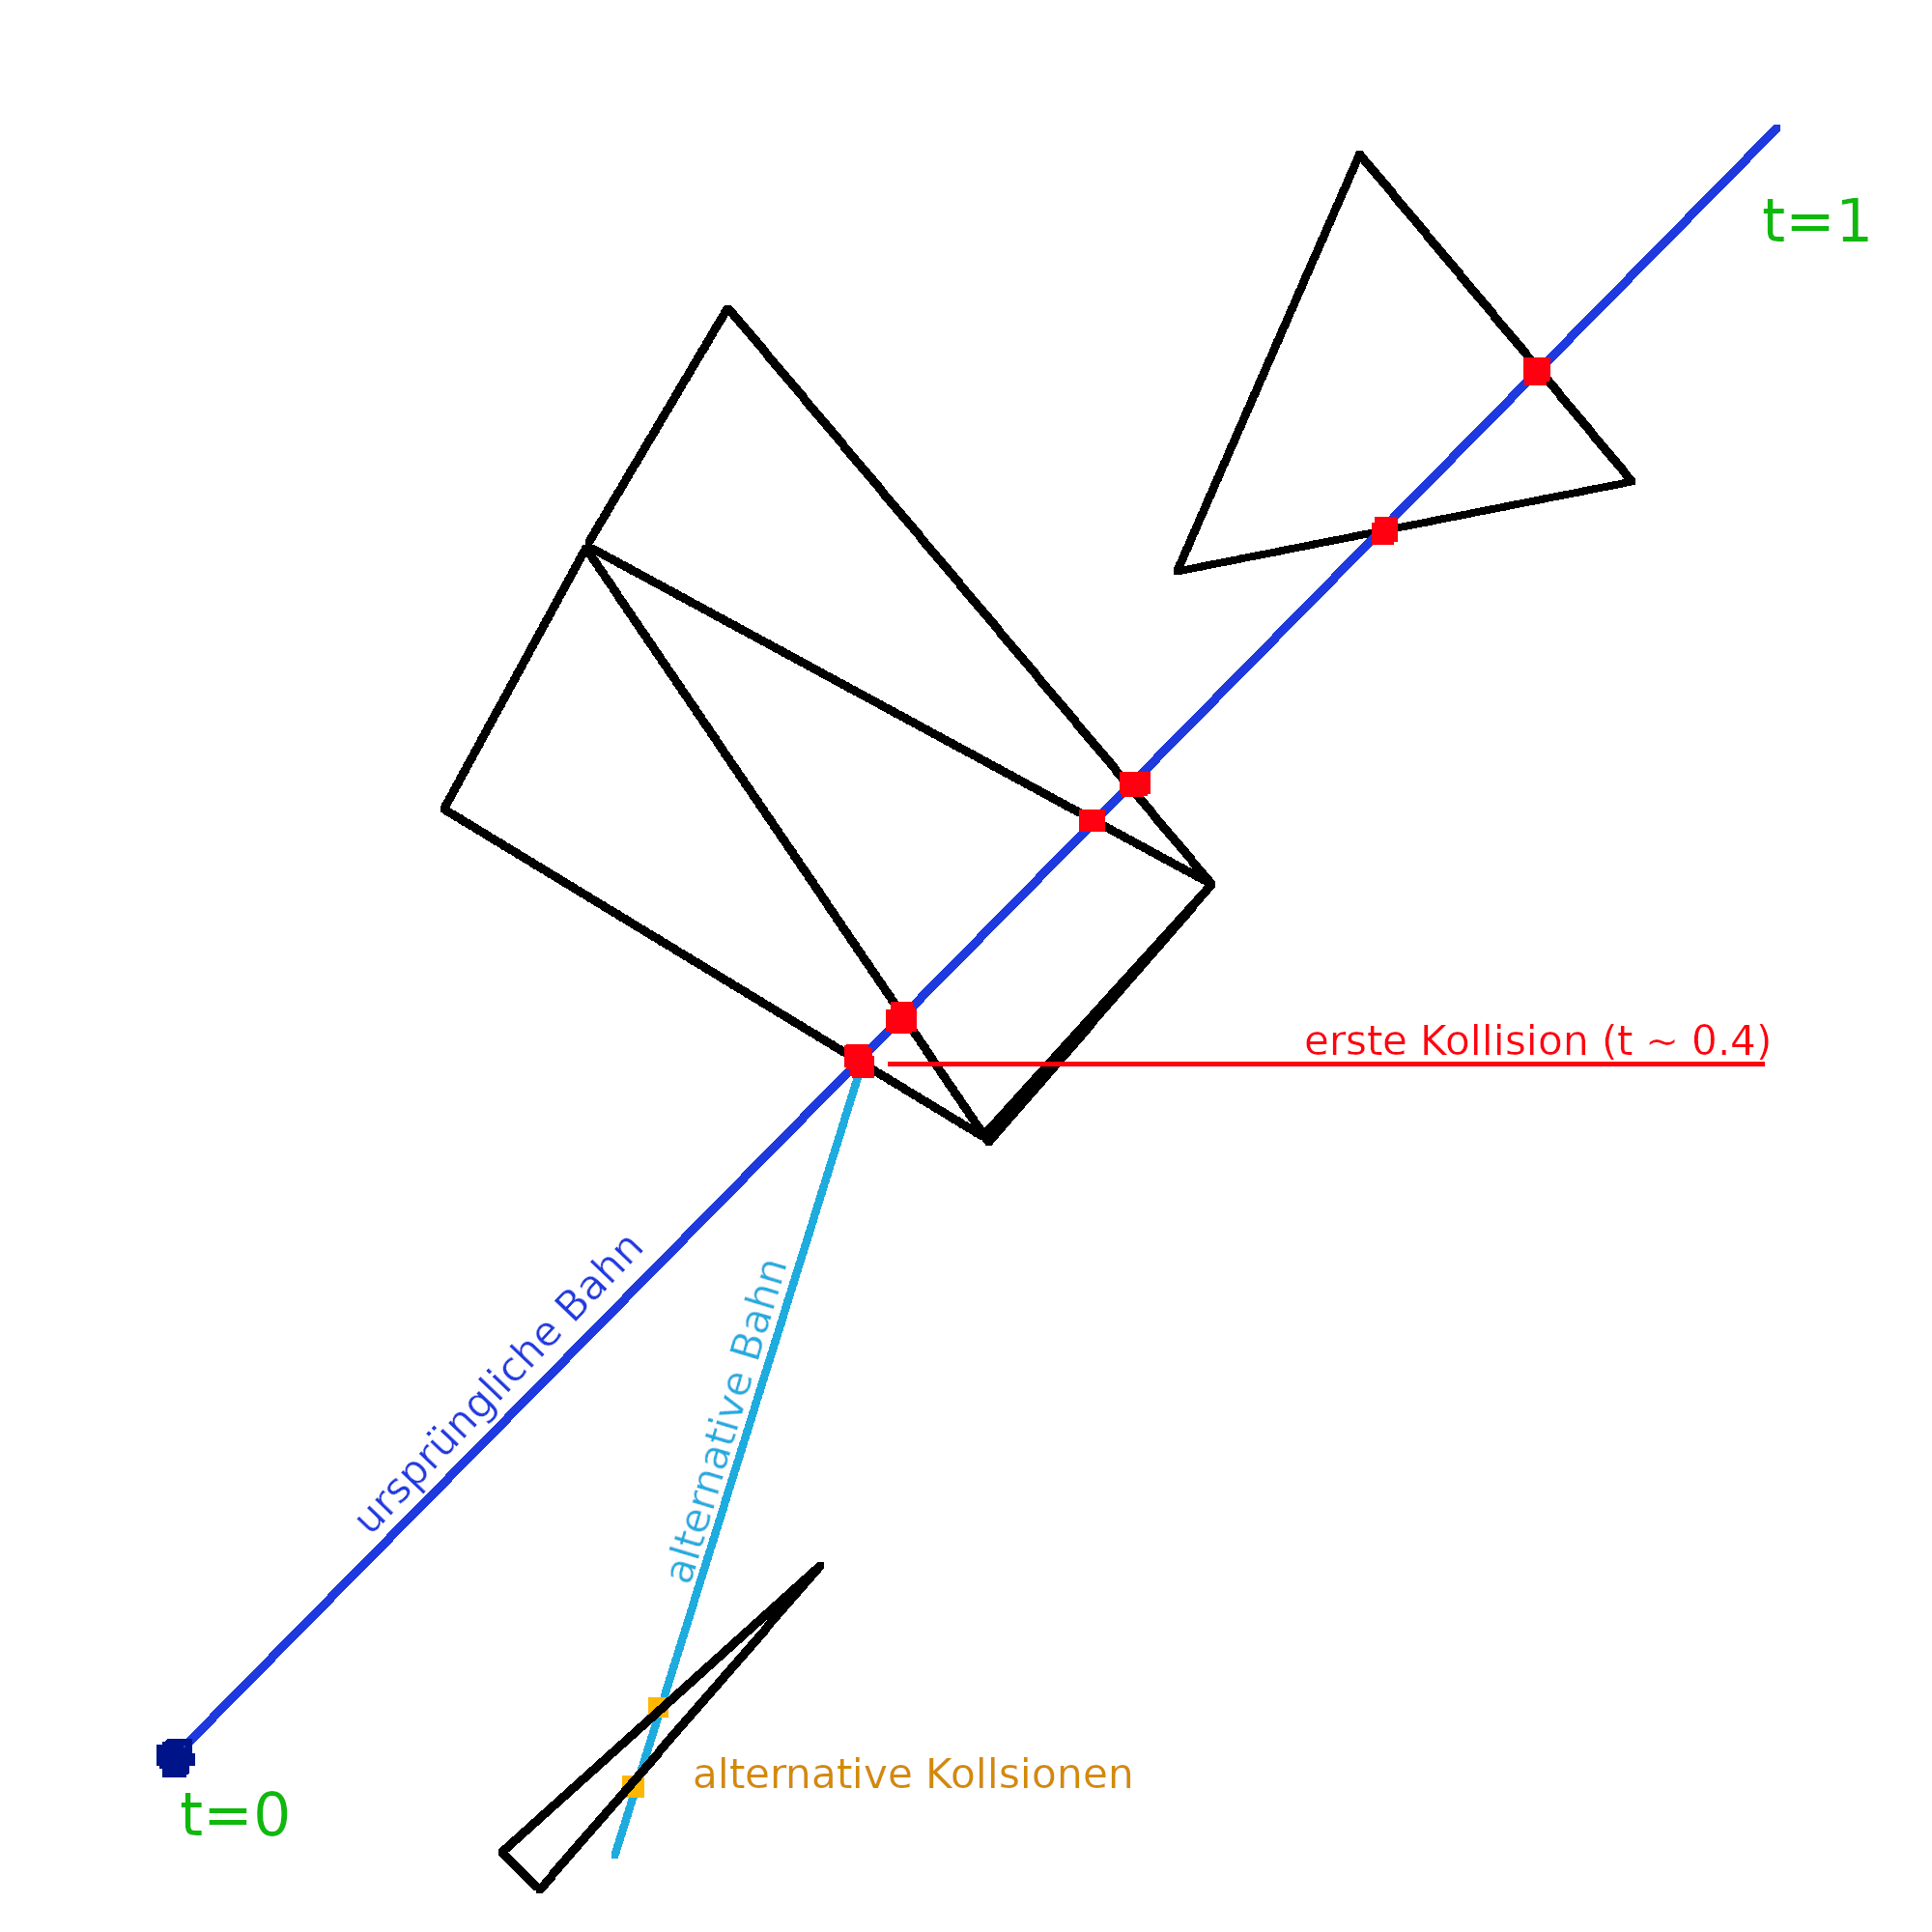
\includegraphics[width=0.6\textwidth]{./res/l3_col.png}
	\caption{2D Kollisionsszenario mit alternativen Bewegungsbahnen eines Projektils an Kollisionskörpern}
	\label{fig:l3col}
\end{figure}
Die Umsetzung der Auflösung von Kollisionen und Mehrfachkollisionen ist explizit aus diesem Projekt ausgeschlossen. Selbst jedoch bei der theoretischen Betrachtung von Mehrfachkollisionen während eines Ticks und Optionen zu deren Auflösung, bzw.~physikalischer Reaktion von Objekten , scheinen vorwiegend Erstkollisionen interessant zu sein. Man vergleiche hierzu Abbildung~\ref{fig:l3col}.\\
An dieser Stelle wird demnach die Annahme getroffen, dass zunächst nur Erstkollisionen durch Intrusion interessanter sind sind und zuerst ermittelbar gemacht werden sollten.


%%TODO look if one can fit that under his hat somewhere, would be rad 
%Ein interessanter Fehler bezogen auf L3 in freier Wildbahn ist in \cite{skyrimwallglitch} zu sehen. Es handelt sich dabei um einen Glitch im Spiel The Elder Scrolls V:Skyrim. Dabei wird eine gleichzeitige Kollision des Spielermodells (welches sich durch eine Ingame-Fähigkeit unüblich schnell bewegt), eines Objekts und einer Wand oder Tür provoziert. Die Kollision, bzw. die wiederholten Kollisionen zwischen dem Spielermodell, dem Objekt (Kessel/Teller/Korb) und der Wand/Tür werden nicht richtig aufgelöst, was dazu führt, dass der Spieler durch die Wand laufen kann.\\


\subsection{Intrusionsermittlung durch lineare Interpolation der Objektbewegung}
Um das Problem zu vereinfachen wird die zunächst die Rotation von Objekten vernachlässigt.\\
Genauer: In diesem Kontext erfährt ein Objekt $o\in OBJ$ während eines Ticks $\delta_i$ keine zeitliche Änderung der Rotation $\forall t \in \Upsilon_{\delta i} : \omega(o, t) = (0,0,0)$. Dies hat mehrere Gründe:
\begin{enumerate}
\item Objekte hielten zum Start des Projekts noch keine Repräsentation für Rotation.
\item Rotation mit einzubeziehen wurde zu Anfang schon als schwierig eingestuft. Dieser Verhalt sollte sich später bestätigen.
\item Es gibt genügend Kollisionsszenarien/Verwendungszwecke für denen Rotation keine Rolle spielen muss. (Logische Kollision, Punktförmige Objekte, unbewegliche Objekte wie z.B. oft Terrain, Verwendungszwecke mit hoher Fehlertoleranz)
\item Es wird ein Experiment der Vernachlässigung von Rotation durchgeführt. Es soll dabei beantwortet werden, ob auch ohne Behandlung der Rotation eine ausreichend zufriedenstellende Illusion von physikalischem Realismus geschaffen werden kann.
\end{enumerate}

Wie in Abschnitt~\ref{sec:objects_sim} bereits beschrieben sind die zeitlichen Änderungen (Geschwindigkeit $v$ und Drehgeschwindigkeit $\omega$) eines Objektes während eines Ticks konstant. Durch die Vernachlässigung der Drehgeschwindigkeit $\omega$ kann die zeitliche Änderung eines Objektes $o$ allein auf Bezug zu Geschwindigkeit $v$ und der Zeit $t$ beschrieben werden, bzw.~alle im Objekt $o$ enthaltenen Punkte $p \in G_o$ beschreiben lineare, parallele Flugbahnen während des Ticks $\delta_i$:
$$l_p = \{p + (t - t_0) * v(o, t_0) | t_0 \leq t \leq t_1\}; X \subseteq \mathcal{F}^3:\{l_p|p\in X\} = \{X| t \in \Upsilon_{\delta_i}\}$$,
 die in ihrer Gesamtheit also das durchlaufene Volumen des Objekts beschreiben:
$$\{l_p|p\in G_o\} = \{G_{o, t}| t \in \Upsilon_{\delta_i}\}$$

Dies ermöglicht die Ermittlung von Kollisionen von Objekten $o_0, o_1$ durch lineare Interpolation der Zeit.\\
Die Eigenschaft der Linearität hat dabei noch den weiteren entscheidenden Vorteil, dass bei einer Relativierung der Objekte wechselseitig zueinander, eine Operation der einer Transformation in Form einer Translation gleichkommt, die Linearität weiterhin gewahrt bleibt. Zum Vergleich: Mit aktiver Rotation beschreiben Objekte relativ zueinander Kurvenflugbahnen.\\
Essenziell zu überprüfende Merkmalspaare $\in \{Area, Edge, Vertex\}^2$ sind:
		\begin{itemize}
			\item [$\{Vertex, Area\}$] Eine Ecke durchschlägt eine Fläche.\\
				$\Rightarrow$ Zu überprüfende Paare: $(V_{o_0}\times A_{o_1})\times (V_{o_1}\times A_{o_0})$
			\item [$\{Edge, Edge\}$] Kanten durchschneiden sich gegenseitig.
				$\Rightarrow$ Zu überprüfende Paare: $(E_{o_0}\times E_{o_1})\times (E_{o_1}\times E_{o_0}) = (E_{o_0}\times E_{o_1})$
		\end{itemize}
		Alle anderen Kombinationen sind entweder in diesen beiden enthalten (z.B. $\{Vertex, Edge\}$ in 1.) oder ein Ereignis dieser beiden Szenarien muss logisch vorher passieren (z.B. 1. oder 2. muss vor $\{Edge, Area\}$ bereits passiert sein).
\ \\
		Aufgrund der Relativierung muss nur eines der Merkmale muss eine zeitliche Bewegung durchführen
		\begin{itemize}
			\item [$$\{Vertex, Area\}$$] 2 Möglichkeiten:
				\begin{itemize}
					\item[Option0:] Eckpunkt $v \Rightarrow$ Linie $l_v$
					\item[Option1:] Dreiecksfläche $a \Rightarrow$ Schiefes Prisma $ \{l_p | p \in \mathcal{A}(a)\}$
				\end{itemize}
				Gewählt wird Option0, da einfachere Berechnung.
			\item [$\{Edge, Edge\}$] Kante $e \Rightarrow$ Parallelogramm $\{l_p | p \in \mathcal{E}(e)\}$
		\end{itemize}
\ \\
		Geometrische Eigenschaften nun beteiligter Formen:
		\begin{itemize}
			\item [Linie] $L = \{p_l | x\in\mathcal{F} ; p_{l0}, p_{l1} \in \mathcal{F}^3 ; p_l = p_{l0} + x * p_{l1}; 0\le x\le 1 \}$
		\item [Dreieck] $T = \{p_t | x,y \in\mathcal{F};  p_{t0},  p_{t1},  p_{t2} \in \mathcal{F}^3; p_t = p_{t0} + x*p_{t1} + y*p_{t2}; 0\le (x+y) \le 1\}$
			\item [Parallelogramm] $P = \{p_p | x,y \in\mathcal{F}; p_{p0}, p_{p1}, p_{p2} \in \mathcal{F}^3; p_p = p_{p0} + x*p_{p1} + y*p_{p2}; 0\le x\le 1; 0\le y\le 1\}$
		\end{itemize}
\ \\
		Beide Szenarien können über Gleichungssysteme zur Ermittlung von Ort- und Zeitkoeffizienten in konstanter Zeit überprüft werden:
		\begin{itemize}
			\item [$\{Vertex, Area\}$] $p_{l0} + x * p_{l1} = p_{t0} + y*p_{t1} + z*p_{t2}$\\
				$x$ ist zudem hier der Koeffizient der Zeit, da die Linie in der Zeitdimension liegt.
			\item [$\{Edge, Edge\}$] $p_{l0} + x * p_{l1} =  p_{p0} + y*p_{p1} + z*p_{p2}$\\
				Sei die ursprüngliche Kante, aus dem das Parallelogramm generiert wurde $\{p_0+y*p_1\}$, so liegt die andere Kante $\{p_0 + z*p_2\}$ in der Zeitdimension und somit ist hier z der Zeitkoeffizient.
		\end{itemize}
\ \\
		Komplexität: $|V_{o0}|* |A_{o1}| + |V_{o1}|*|A_{o0}|$ + $|E_{o0}| * |E_{o1}|$

		\begin{itemize}
			\item Zuverlässige Ermittlung der Erstkollision durch Findung des minimalen Zeitkoeffizienten.
			\item Mathematisch exakte Ermittlung der Zeit einer Kollision durch Zeitkoeffizienten.
			\item Mathematisch exakte Ermittlung des Orts einer Kollision durch Ortskoeffizienten.
			\item Ermittlung der Beteiligen Objektmerkmale der Erstkollision.
		\end{itemize}
Wie beschrieben kann dieses Verfahren bereits in einigen Szenarien, bei denen Rotation keine Rolle spielt, als vollständige Lösung zum Einsatz gebracht werden.\\
Es bleibt das Experiment, eine Illusion physikalischer Vorgänge mit rigider Körperkollision über den Linearen-Interpolationsalgorithmus zu realisieren.\\
Zunächst scheint dabei klar: Durch die Vernachlässigung der Rotation passieren physikungetreue Fehler, besonders, je größer die Varianz des Abstands der vom Objekt enthaltenen Punkte zum Objektursprung ist. Objekte sind dann unförmig und durchstreifen bei zeitlicher Bewegung logisch ein zu einem gewissen Grad anderes Volumen, als der lineare Interpolationsalgorithmus annimmt. Diese Diskrepanz kann sowohl zu False-Positives als auch zu False-Negatives führen.\\
Des Weiteren muss die vernachlässigte Rotation nachgeholt werden. Durch einen Extremfall dieser Nachlässigkeit fällt ein weiteres Defizit des Algorithmus auf. Ist die relative Geschwindigkeit zweier Objekte $=0$, wird aus Sicht des Algorithmus' kein Volumen durchstriffen. Es werden zwischen diesen Objekten dann gar keine Kollisionen erkannt, welche durch Rotation logisch/visuell aber auftreten.\\
Man versucht diese Problem durch statische Kollisionstests am Tickende zu lösen. Dabei wird die akkumulierte Rotationsbewegung/Rotationstransformation auf einmal ausgeführt. Vor und nach der Bewegung wird statisch eine Kollisionsabfrage berechnet.\\
Diese Anpassung bringt eigene Probleme mit sich:
\begin{enumerate}
\item Durch die akkumulierte Drehung kann eine Kollision bei schnellen Drehgeschwindigkeiten durch nur die Tests am Anfang und am Ende des Ticks komplett übersehen werden.
\item Nach der Rotationtransformation können Objekte sich in einem gegenseitigen Schnittzustand $D(o_0, t_1)\cap D(o_1, t_1) \neq \emptyset$ befinden, da an dieser Stelle keine Intrusion erkannt werden kann. Der Zustand könnte durch einen Linearen-Interpolationsalgorithmus zwar erkannt werden, jedoch sind bis dato im Projekt keine Möglichkeiten enthalten, vernünftig auf diesen Fall zu reagieren.
Eine Idee ist die Suche nach einem Zeitpunkt vor der Überschneidung, durch beispielsweise Bisection des Drehungsausschlags. Es erscheint jedoch, dass der wiederholte Aufwand durch Transformation und Ausführen des Interpolationsalgorithmus in der gegebenen Zeit ebenfalls keine Qualitativ hochwertigen Ergebnisse erzielt. Der Schnittzustand wird zudem in der rigiden Körperkollision als fehlerhafter Zustand angesehen, den die Kollisionsroutine eigentlich verhindern soll.
\end{enumerate}

%%TODO glitchpic

Es wird also weiter nach Lösungen gesucht, die sich dem Rotationsproblem besser annehmen.

\subsubsection{Gilbert-Johnson-Keerthi-Distanzalgorithmus (GJK)}
GJK ist ein Algorithmus, der zwischen kompakten, konvexen Mengen $K_0, K_1 \subseteq \mathbb{R}^3$ die minimale euklidische Distanz $distance(K_0, K_1) = min\{|k_0 - k_1| | k_0\in K_0 ; k_1 \in K_1\}$ errechnet. Er wurde 1988 publiziert \cite{gjk} und scheint heute gerne in Videospielen verwendet zu werden. Beispiele sind dabei Blizzard Entertainments Diabolo 3 \cite{gdc-physics} und Valves Half-Life 2\cite{gjk-blog}.\\
Im Folgenden wird Die Urquelle \cite{gjk} gibt den Algorithmus im mathematischen Kontext an. Die Umwandlung der Mathematik in eine gute Maschinenimplementierung wird nicht als trivial eingeschätzt. Es fehlen die nötigen Erfahrungswerte mit dem Algorithmus. Es werden daher weitere Quellen mit praktischem Fokus zu Rate gezogen, um die Implementierung umzusetzen \cite{gjk-blog}\cite{gjk_vid}.
Im GJK-Algorithmus sollen Eigenschaften der sogenannten Minkowski-Differenz $\mathcal{M}:\mathcal{P}(\mathbb{R}^3)^2\mapsto \mathcal{P}(\mathbb{R}^3); \mathcal{M}(K_0, K_1) = \{a - b| a\in K_0 ; b\in K_1\}$ \cite[p.195]{gjk} ausgenutzt werden, von der die Relevanten wie folgt lauten:\\
Sei $O = (0,0,0)$ der Koordinatenursprung.
	\begin{enumerate}
		\item Die Minkowski-Differenz zweier konvexer Körper ist ebenfalls konvex \cite[p.195]{gjk}.
		\item $K_0 \cap K_1 \neq \emptyset \Rightarrow \exists a_o, b_o \in K_0 \cap K_1, a_0 \in K_0, b_0 \in K_1 : a_o = b_o \Rightarrow a_o - b_o = O \Rightarrow O \in \mathcal{M}(K_0, K_1)$
		\item $K_0 \cap K_1 = \emptyset \Rightarrow \forall a_o\in K_0, \forall b_o\in K_1 : a_o \neq b_o \Rightarrow a_o - b_o \neq O \Rightarrow O \notin \mathcal{M}(K_0, K_1)$.
		\item $distance(O, \mathcal{M}(K_0, K_1)) = distance(K_0, K_1)$
		\item (2.) $\wedge$ (3.) $\wedge$ (4.) $\Rightarrow K_0 \cap K_1 \neq \emptyset \Leftrightarrow O \in \mathcal{M}(K_0, K_1)	\Leftrightarrow distance(K_0, K_1) = 0$	
		\item (4.) $\Rightarrow distance: \mathcal{P}(\mathbb{R}^3)^2 \mapsto \mathbb{R}^+_0$ (gibt nur positive Distanzen aus)
	\end{enumerate}
	Man bemerkt: Das Verfahren behandelt das Schnittproblem, statt des Intrusionsproblems. Durch die Fähigkeit des GJK-Algorithmus, die Distanz zwischen zwei Objekten zu ermitteln, ist dieser jedoch ein praktisches Werkzeug auch um das Intrusionsproblem ebenfalls zu lösen.
Zum Beispiel ist ein Ansatz mit GJK, durch Abstraktion über einer Nullstellensuche der Distanz zwischen zwei Objekten das Intrusionsproblem zu abzubilden (vgl.~Eigenschaft 5, vgl. \cite{gdc-physics}).\\
GJK eignet sich also für dieses Projekt und soll implementiert werden. 

Zunächst muss die Eingabeinformation von kompakten, konvexen Punktmengen, die der Algorithmus fordert, äquivalent hergestellt sein, um sicherzustellen, dass der Algorithmus auch mit Polygon-Meshes durchgeführt werden kann. Für diese ist allerdings keine Konvexität gefordert und eine entsprechende kompakte Repräsentation nicht gegeben.
Zunächst soll Konvexität hergestellt werden. Definierte nicht-konvexe Objekte können in Konvexe Partitionen aufgeteilt werden. Jede Partition zählt dann als eigenes Objekt gegenüber dem Algorithmus. Das erhöht die erwartete Komplexität der gesamten Kollisionsroutine mit GJK um den Grad der Partitionierung.\\
\ \\
Es wurde zu einer automatisierten Methode recherchiert, um die Partitionierung herzustellen. Insbesondere die minimale Partitionierung scheint hier von Interesse, um die Erhöhung der Komplexität zu mitigieren.\\
Zusätzlich zu eigenen Überlegungen bestätigen die Quellen \cite{ARTIGAS20111968} und \cite{grelier2019minimum} die NP-Vollständigkeit, bzw. NP-Härte zusammengehöriger Probleme der minimalen konvexen Partitionierung.\\
Eine nicht minimale Partitionierung wäre zunächst auch ausreichend und auch lange Berechnungszeiten zur Partitionierung würden für rigide Objekte nur einmaligen Aufwand zum Programmstart bedeuten und wären daher nicht kritisch.\\
Bei Versuchen, Algorithmen für dieses Problem zu erstellen, wird jedoch eine weiter klare Hürde erkenntlich: Allein durch die Polygon-Mesh, sind Innen und Außenseite des Objektes prinzipiell nicht definiert.\\
Für grafische Zwecke kann dieser Bezug oft durch das sog. \textit{Winding} eines Dreiecks angegeben werden. Dabei wird die Reihenfolge der Angabe der Ecken eines Dreiecks konventionell festgelegt, wodurch die Richtung der Flächennormale eines Dreiecks kontrolliert werden kann, die dann Außen oder Innenseite spezifiziert. Auch die direkte Angabe einer Flächennormale zu jedem Dreieck (oder sogar jedem Eckpunkt) is im graphischen Kontext für bestimmte Effekte gebräuchlich. Diese Konzepte werden grafisch im Projekt jedoch bis dato nicht verwendet und sind daher auch nicht vorhanden.\\
Eine Konvention für ein \textit{Winding} wurde allerdings im Projekt eingeführt, nicht zuletzt, da diese die Implementierung des GJK vereinfacht.\\
Für die in dieser Projektarbeit verwendeten Testzwecke erscheint der Aufwand der Automatisierung der konvexen Partitionierung für dieses Projekt letztendlich doch zu hoch und thematisch zu fremd.\\
\ \\
Die konvexe Partitionierung des Objektes $o$ wird daher manuell und explizit bei Modellen durch die Angabe von Mengen von Indices von zueinander konvexen Eckpunkten $P_i \subseteq V_o$ angegeben.
Zusätzlich ist die Äquivalenz zur kompakten Punktemenge $K_o$ gefordert. Diese ist nun implizit durch die Konvexität gegeben. $K_o$ ist konvex, wenn gilt $\forall p_0, p_1 \in K_o, \forall x \in [0,1] : p0 + x * (p_1 - p0) \in K_o $. In Mesh-Repräsentation $G_o$ sind nicht alle diese Punkte enthalten. Jedoch, wenn $K_o$ konvex so sind die Hüllen $\mathcal{H}(K_o) = \mathcal{G_o}$ ebenfalls konvex. Alle Punkte $K_o \backslash G_o$ können so durch die Konvexitätsdefinition impliziert werden. Die zusätzlich mit der Objektrepräsentation mitgelieferte Partitionierung erweitert also die verfügbare Information und schafft in dieser Hinsicht Äquivalenz zwischen Polygon-Meshes und kompakten Mengen und die Unterscheidung von Innen und Außen. Informationen zu verbundenen Ecken einer Polygon-Mesh $I_o$ werden dadurch in diesem Kontext ebenfalls redundant. Der Algorithmus kann demnach außschließlich unter Einbeziehung von Eckpunkten $V_o$ verfahren.\\
Durch die Feststellung der Äquivalenz wurde ermittelt, dass eine Variante des GJK-Algorithmus auch an Polygon-Meshes durchgeführt werden kann.\\
Es kann also eine Diskretion/Beschränkung auf die Information der Eckpunkte der Polygon-Mesh $V_o$  verwendet werden, was vorteilhafte Iterationslängen im Algorithmus zur Folge hat ($V_o \ll G_o \ll K_o$).

%%TODO refactor and actually provide the images
Eine Illustation einer diskreten Minkowski-Differenz ist in den Abbildungen \ref{fig:minkov_col}, \ref{fig:minkov_col_solo} und \ref{fig:minkov_noncol}zu sehen. Zu sehen sind, in Rot und Blau, die 2 Objekte, welche sich in \ref{fig:minkov_col} überschneiden und in \ref{fig:minkov_noncol} nicht. Die Gebilde, deren Ecken grün sind und deren Kanten rot und blau sind sind die jeweiligen Minkowski-Differenzen.
Die grünen Punkte sind alle Punkte, die durch die Anwendung der Minkowski-Differenz auf die Menge der Eckpunkte beider Körper ermittelbar sind.\\
Die Kanten sind rot oder blau, je nachdem von welchem Ursprungskörper eine Kante Einfluss erhält. So ist die Beteiligung beider Körper an der Differenz besser zu erkennen. Theoretisch sind auch die Kanten zwischen jedem Punktepaar mit gemischten Einflüssen der beiden Ursprungsobjekte darstellbar, welche aus Darstellungsgründen nicht in der Grafik enthalten sind. Isoliert steht in Abbildung \ref{fig:minkov_col_solo} die Minkowski-Differenz aus Abbildung \ref{fig:minkov_col}.\\


Eigenschaften der Minkowski-Differenz müssen den Umstand der Diskretion respektierend ausgenutzt werden.\\

\begin{enumerate}
		\item Die diskrete Minkowski-Differenz ist ebenfalls konvex.	
		\item Ein Simplex ist eine durch eine Anzahl $n\in\mathbb{N}$ Eckpunkte $s\in\mathcal{M}(V_{o_0}, V_{o_1})^n$ aufgespannte $n$-dimensionale geometrische, inhärent konvexe Form (hier: Punkt für $n=1$, Gerade $n=2$, Dreieck $n=3$, Tetraeder $n=4$). Durch die Konvexität ist die entsprechende kompakte Menge $K_s$ implizit definiert.
		\item Für das nächste Simplex $s_{nearest} \in \mathcal{M}(V_{o_0}, V_{o_1})$ zum Ursprung $O$ gilt außerdem $distance(O, s_{nearest}) = distance(K_{o_0}, K_{o_1})$ \cite[p. 195]{gjk}. 
		\item $O \in \mathcal{M}(K_{o_0}, K_{o_1}) \nRightarrow O \in \mathcal{M}(V_{o_0}, V_{o_1})$. Jedoch kann eine äquivalente Beziehung gefunden werden: $O \in \mathcal{M}(K_{o_0}, K_{o_1}) \equiv \exists Simplex~s \in \mathcal{M}(V_{o_0}, V_{o_1}) : O \in K_s$, , das den Ursprung enthält/umschließt.

\end{enumerate}

Die Implementierung des GJK bezieht sich also auf die Suche nach dem nähersten, bzw. umschließenden Simplex zum Ursprung.\\
Es wird im Folgenden der Algorithmus beschrieben:
\begin{enumerate}
	\item Initialisiere mit
	\begin{enumerate}
		\item Zwei konvexen (Teil-)Objekten $o_0, o_1$
		\item ihrer diskreten Minkowski-Differenz zu einem Zeitpunkt $\mathcal{M} = \mathcal{M}(V_{o_0}, V_{o_1})$
		\item beliebigem Startpunkt $P_0 \in \mathcal{M}_d$
		\item der Menge von maximal 4 indizierten Simplexeckpunkten $s = \{s_0 = P_0\}$
		\item der Suchrichtung $D = -P_0$
		\item der minimalen gefundene Distanz $d_{min} = \infty$
		\item der Fähigkeit, Abstände zwischen einem Simplex und dem Ursprung zu errechnen $distance: Simplex \times \mathcal{F}^3 \mapsto \mathcal{F} ; distance({}, X) = \infty$
	\end{enumerate}	
	\item Finde neuen Punkt $s_{|s|}$ zur $(|s|+1)$-dimensionalen Erweiterung des Simplex den maximalen Punkt $v \in \mathcal{M}$ in der Suchrichtung $D$ über das Skalarprodukt $s_{|s|} = v \in \mathcal{M} : v \circ D = max\{D \circ v_i ; v_i \in  ßmathcal{M}\}$. Da $\mathcal{M}$ konvex, existiert dieses Maximum in jede Richtung \cite[p. 195]{gjk}.
	\item $-s_{|s|} \circ D > 0 \Rightarrow O \notin \mathcal{M}$. Es könnte $d_{min} = distance(s, O)$ gesetzt werden. Dieser Schritt ist hauptsächlich für einen verfrühten Abbruch interessant, wenn nur ermittelt werden soll, ob ein Schnitt $K_{o_0} \cap K_{o_1} \neq \emptyset$ existiert, oder nicht.
	\item Durch die Punkte $Simplex~s_{new} = s \cup {s_{|s|}}$ kann eine Menge von Simplices $\mathcal{P}(s_{new})$ beschrieben werden. Es soll das zum Ursprung nächste Simplex ausgewählt werden. Die Auswahl $\mathcal{P}(s_{new})$ kann weiter dadurch eingeschränkt werden, dass nur neue Simplices, die durch den neuen Punkt $s_{|s|}$ bekannt wurden überprüft werden müssen, da durch die Suche des Punkts in Suchrichtung $D$ an dieser Stelle eine Distanzverbesserung durch den neuen Punkt erwartet wird. Das Gegenereignis hierzu kann durch Konvexität von $\mathcal{M}$ und der Maximaleigenschaft der Punkte in $s$ ausgeschlossen werden, solange das nächste Simplex nicht bereits erreicht ist \cite{gjk-vid}.  Die reduzierte Menge $S_{check} \subset \mathcal{P}(s_{new}); S_{check} = \{ s \in \mathcal{P}(s_{new}) | s_{|s|} \in s \}$ wird demnach stattdessen überprüft und das neue nächste gefundene Simplex 
	 $s \in s_{check} : distance(s, O) = min\{distance(s', O) | s' \in s_{check}\}$
	 ermittelt.
	\item Falls keine kleinere Distanz gefunden wurde, ist das nächste Simplex zum Ursprung gefunden. $d_{min} \leq distance(s, O) \Rightarrow distance(K_{o_0}, K_{o_1}) = distance(s, O) = d_{min}$ (\textbf{RETURN})
	\item Ist das nächste Simplex ein Tetraeder $|s| = 4 \Rightarrow O \in K_s \Rightarrow distance(\mathcal{M}, O) = 0$ (\textbf{RETURN})
	\item $d_{min} = distance(s, O)$
	\item Die neue Suchrichtung $D = D_{new}(s)$ wird orthogonal zum Simplex $s$ in Richtung des Ursprungs festgelegt. Die konkrete Berechnung hängt dabei von $|V'|$ ab. Ein Beispiel ist: $|s| = 2 \Rightarrow D(s) = (b-a)\times (O-a)\times (b-a);  \{a, b\} = s$, mit $\times$ als Kreuzprodukt zweier Vektoren.
	\item Wiederhole ab 2.
\end{enumerate}
Rückgabewerte sind immer $d_min$ \& $s$.
Es werden Implementierungsspezifika und aufgetretene Probleme geschildert:\\
\begin{enumerate}
\item Für die Berechnung von Minkowski-Punkten $\mathcal{M}(V_{o_0}, V_{o_1})$ wurde ein Generator implementiert, der zum Minkowski-Punkt die Indices der Verwendeten Eckpunkte der Ursprungsmodelle $V_{o_0}$ und $V_{o_1}$ mitführt. Damit können durch den Erhalt des nächsten Simpex $s$ die Beteiligten Merkmale/Simplices and den Ursprungsobjekten ermittelt werden.
\item Die Quelle \cite{gjk-vid} ist zunächst primär für die Struktur des Implementierungsversuchs. Die dort gezeigte Implementierung funktioniert angeblich alleinig auf Basis der Abbruchkriterien in 3.~(verfrühter Abbruch) und 6.~ ohne 5..
Die Grafik \ref{fig:why_criteria} zeigt dabei einen Widerspruch, dass das vorgeschlagene Abbruchkriterien in 3. und 6. nicht ausreicht um ein nächstes Simplex zum Ursprung zu erreichen und die minimale Distanz zu ermitteln.\\
Dort zu sehen ist das schwarze Dreieck $\Delta ABC$ und der grüne Ursprung $O$. Angenommen der Algorithmus beginnt an Punkt $B$ und sucht in Richtung des Ursprungs $D = \vec{BO} = -\vec{B}$ so wird als nächster Simplexeckpunkt $s_{|s|} = A$ gewählt und somit $s_{new} = \bar{BA}$ gefunden. Das Abbruchkriterium prüft nun, ob der Ursprung noch hinter diesem maximalen Punkt in der Suchrichtung läge, was durch $ -\vec{A} \circ -\vec{B} > 0$ festgestellt wird. In dem in der Grafik gezeigten Szenario führte dies zum Abbruch. Das gefundene Simplex $\bar{AB}$ ist jedoch nicht das nächste am Ursprung. Das ist stattdessen die Linie $\bar{AC}$.\\
Unter Umständen ist es die undokumentierte Intention der Quelle \cite{gjk-vid} nur eine Implementierung zu liefern, die keine minimale Distanz oder nächste Simplices ermittelt, sondern nur ob ein Schnitt existiert, oder nicht. Die Ausschreibungen der Quelle als Implementierung des GJK-Algorithmus ist daher etwas irreführend, erleichterte jedoch den Einstieg in die Materie.
\item Die ungenügende Implementierung wurde daraufhin auf die Anforderungen von Distanz- und Simplexfindung unter Zuhilfenahme von Quelle \cite{gjk} angepasst.
Bei der Anpassung wurde zunächst mit Abbruchkriterien experimentiert um den im Schritt 4.~gezeigten Brute-Force-Aufwand der minimalen Distanzberechnungen zu vermeiden. Vorschläge sind:
\begin{enumerate}
	\item Die hier als Status-Quo vorgestellte Brute-Force-Distanzberechnung in Schritt 4.~und anschließende Auswertung in Schritt 5..
	\item Statt Schritt 5.:
	 $$s_{|s|} \in s \Rightarrow distance(K_{o_0}, K_{o_1}) = distance(s, O) = d_{min}\text{(\textbf{RETURN})}$$ : Neue Simplexpunkte $s_{|s|}$ sind nach Schritt 2.~ maximal in einer Suchrichtung $D$, die in Richtung des Ursprungs liegt. Ist das nächste Merkmal erreicht, so wird nach Schritt 4.~in eine Richtung gesucht, deren maximale Punkte bereits bekannt sein müssen. Daher ist ein mögliches Abbruchkriterium: Abbruch beim finden eines Support-Punktes, der bereits bekannt ist. $\mathcal{O}(3)$, da in Schritt 4.~immer gilt:$|s|\leq 3$
	 \\TODO-------------------------------------
	\item Ein neuer Support Punkt soll eine Erweiterung in die Suchrichtung darstellen. Seien $S$ die bekannten Support-Punkte und $P_{\#S}$ der neu gewonnene. Nehmen wir die Suchrichtung als Ebenennormale an, liegt das von den in $S$ enthaltenen Punkten gebildete Simplex in der dieser Ebene. Alle neuen Punkte, welche eine Erweiterung in Richtung des Ursprungs darstellen sollen, müssen in Richtung der Ebenennormale liegen. Dies ist festzustellen, in dem Vektoren $V := P_{\#S}-s_i ; s_i\in S$ auf ein positives Skalarprodukt mit der Suchrichtung überprüft werden. Abbruchkriterium: $\exists V : D \cdot V <= 0$. Idee: Wird ein koplanarer oder gar schon bekannte Support-Punkt gefunden ist das Skalarprodukt $0$ und der Abbruch wird eingeleitet, da keine Erweiterung mehr schaffbar ist.
\end{enumerate}
Bei Versuchen mit den Abbruchkriterien (b) und (3) wurden jedoch Probleme erkennbar konvergierte der Algorithmus regelmäßig nicht. Es wurden folgende Fehler gefunden:

\end{enumerate}



\begin{figure}
	\centering
	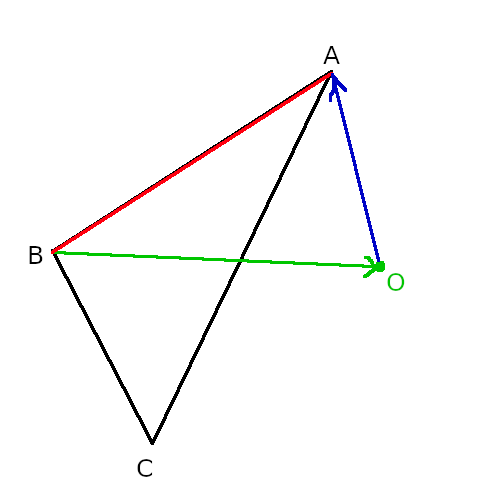
\includegraphics[width=0.6\textwidth]{./res/why_criteria.png}
	\caption{Szenario, in dem das gezeigte Abbruchskriterium nicht am nähesten Merkmal zum Ursprung stoppt.}
	\label{fig:why_criteria}
\end{figure}

\begin{enumerate}
	\item Falsche Annahme: Das näherste Merkmal der Markovsumme ist eindeutig.\\
	Generierbare Simplices in der Markovsumme können überlappen (z.B. aber nicht ausschließlich mit anteilig gleichen Eckpunkten bei Dreiecken). Es können demnach mehrere nächste Simplices zum Ursprung existieren.\\

\begin{figure}
	\centering
	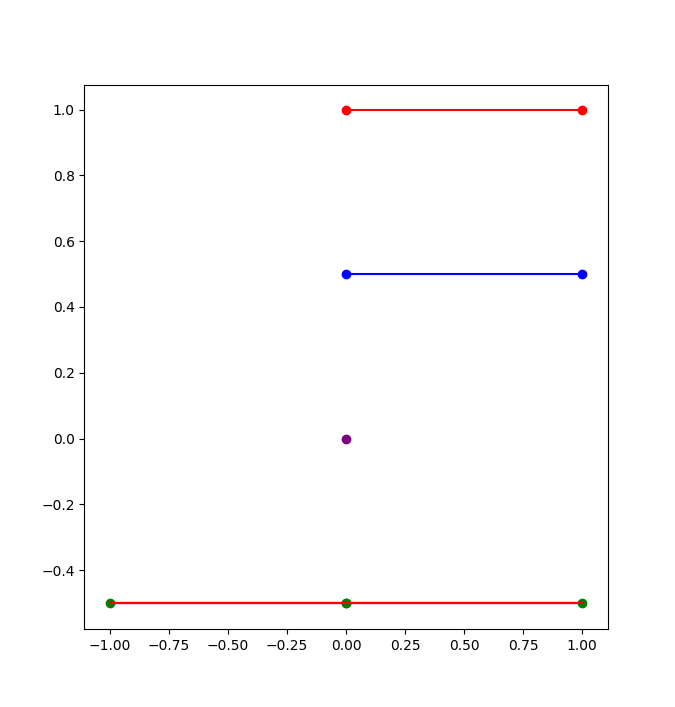
\includegraphics[width=0.6\textwidth]{./res/parallel_features.png}
	\caption{Szenario, in dem das gezeigte Abbruchskriterium nicht am nähesten Merkmal zum Ursprung stoppt.}
	\label{fig:parfeat}
\end{figure}

		Die Grafik \ref{fig:parfeat} zeigt ein solches Szenario. Oben im Bild, die rote und blaue Linie, geben die Ursprungsobjekte an. Der Ursprung ist in violett zu sehen. Die unten im Bild befindliche Linie ist die Markovsumme der roten und blauen Linie. An dieser zu sehen, in Grün, sind die generierten Eckpunkte. Die koplanarität erlaubt dem Algorithmus das Ignorieren des mittleren grünen Punktes. Demnach sind hier der mittlere Punkt und die Linie, welche die beiden äußeren Punkte verbindet exakt gleich weit vom Ursprung entfernt, genauso sind die Linien von jeweils einem Punkt von außen zur Mitte, und ein Dreieck aus allen grünen Punkten.

	\item Falsche Annahme: Verwendete Funktionen sind ausreichend genau.\\
		Theoretisch sollten (nahezu) koplanare Merkmale dieselbe neue Suchrichtung erzeugen. Daraufhin neu gefundene Support-Punkte sind deterministisch (Reihenfolge der Markovpunkte in der Maximumssuche ist immer gleich, Maximumssuche ebenfalls deterministisch). Ungenauigkeiten bei der Suchrichtungsermittlung arbeiten jedoch diesem Determinismus entgegen und erzeugte bei (unter floating Point präzision) nahezu gleichen Eingaben unterschiedliche Punkte, wenn eine auswahl von nahezu koplanaren Punkten existiert. Mehr noch: Alle neuen Punkte skalierten dabei regelmäßig auf Grund der Ungenauigkeit auch noch positiv mit der Suchrichtung was zur Folge hat das Abbruchkriterien 2 und 3 zu keiner konvergenz führten und den Worst Case einer Endlosschleife annehmen.\\
	Die Ungenauigkeit wurde auf die Kondition des Kreuzproduktes zurückgeführt, welches hauptsächlich zur Ermittlung der orthogonalen Suchrichtung verwendet wird. Das ursprüglich als zu komplex angesehene Abbruchkriterium 1 arbeitet nicht mit der aus Kreuzprodukten erzeugten Suchrichtung, sonder direkt auf den bekannten Merkmalen, verwendet selbst keine Kreuzprodukte und wird daher die einzig verbleibende Option. Das Kriterium führte auch in allen Tests erfolgreich zur Konvergenz.
\end{enumerate}
~\\
Weiter ist der Algorithmus bis jetzt nur ein statischer Intersektionstest. Um aus dem Schnittalgorithmus einen Intrusionsalgorithmus zu machen, wird eine Nullstellensuche auf die erhaltene Distanz angewandt.
Das Wurzelsuchverfahren hat zudem den Vorteil, dass es unabhängig von der Bewegungsart der Objekte ist. Animation, Rotation oder beliebige Transformation ist prinzipiell denkbar, solange über eine stetige Distanzfunktion abstrahiert wird.\\
Insbesondere im Falle der Rotation sind Überlegungen zu Startpunkten der Suche and der Distanzfunktionskurve anzustellen. Bei einer schnellen Rotation kollidieren Objekte unter Umständen mehrfach hintereinander, mit kollisionsfreien Episoden dazwischen. Bei Betrachtungen der Intrusion können Nullstellen sowohl beim Ein- als auch beim Austritt festgestellt werden.\\
Die Distanzfunktion verhält sich bei rotierenden Körpern wie eine Schwingung. Es gilt das Nyquist-Shannon-Abtasttheorem. Um beispielsweise die erste Nullstelle/Kollision zu finden ist die Rotationsgeschwindigkeit eines Objektes von Bedeutung, um den Suchraum bedeutend einzugrenzen.\\
Desweiteren ist an dieser Stelle festzustellen, dass das Verfahren wieder durch die Rotationsgeschwindigkeit beschränkt wird.
\\
Des weiteren bleibt ein Problem mit der Restriktion auf konvexe Objekte mit diesem Ansatz. 
Nicht-konvexte Objekte können in konvexe Objekte aufgetrennt werden. Praktisch wird diese Trennung meist extra mit dem Modell angegeben. Dabei sind in der Industrie die Form des tatsächlichen Modells und den zur Kollision angebenen Formen oft nicht kongruent und stellen daher inakkurate Hitboxen dar.\\
Automatisierte Methoden der Aufteilung sind komplex. Prinzipiell, für den Fall dass Objekte rigide sind, ist eine solche Aufteilung 1-mal Aufwand und daher Echtzeitfähig. Sind Objekte jedoch flexibel, z.B. durch Animation an Gelenken, müsste eine automatisierte Aufteilung bei jeder Änderung, u.U.~ mehrere male pro Tick auf ein Objekt angewendet werden. Das wäre Echtzeitfähig nicht tragbar. Deshalb werden in vielen Videospielen Gelenke ignoriert oder durch Kugeln approximiert.\\
Eine Familie nicht-konvexer Objekte, welche aus konvexen Objekten aufgebaut ist, ist prinzipiell noch abdeckbar. Dabei ist wiederholtes Verwenden des GJK-Algorithmus für jedes Teilobjektepaar verschiedener Ursprungsobjekte vonnöten. \\
Es lohnt sich, konvexe Teilobjektpaare durch andere Verfahren vorzufiltern und auszuschließen, wenn möglich.\\
Möglicher Ansatz hierfür ist z.B.~ wieder AABB-Pruning (wir bereits aus L1 bekannt).
\\
Überprüfung der erfüllung gestellter Anforderungen aus L3:\\
\begin{itemize}
	\item Die Kollision wird ermittelt
	\item Die Kollisionszeit wird in einem bestimmten Genauigkeitsrahmen während der Wurzelsuche bekannt.
	\item Die beteiligten Merkmale können aus den ermittelten nähersten Supportpunkten zurückgerechnet werden. Dazu werden zu den Supportpunkten die Quellpunkte mitgeführt.
\end{itemize}

Für das GJK-Wurzelverfahren wird ein Fazit gezogen:
\begin{itemize}
	\item abstrahiert erfolgreich das Intrusionsproblem durch die Distanz für beliebige stetige Bewegungen oder gar Objektveränderungen
	\item fordert Aufteilung in konvexe Objekte
	\item Wurzelsuche optimierbar oder erweiterbar durch weitere Verfahren (vgl. \cite{gdc-physics})
	\item Verwendbar in vielen weiteren Kollisionsverfahren, in denen Distanz ermittelt werden muss
\end{itemize}
%TODO Complexity

Weitere Anmerkungen zum GJK-Algorithmus.
Der Kernpart des GJK-Algorithmus behandelt das Schnittproblem in beliebigen Dimensionen. Denkbar ist daher die Verwendung des GJK bei 4-dimensionalen Objekten, wie sie bei der linearen Interpolation behandelt wurden. Generell ist dieser Part des GJK im O-Kalkül sogar schneller als die $O(m*n)$ der linearen Interpolation. Die Informationen über beteiligte Features und vor allem, der konkrete Zeitpunkt der Kollision gehen dabei allerdings verloren. In bestimmten Szenarien\\
Es gibt noch zahlreiche andere Algorithmen, welche den GJK-Algorithmus verwenden um Situationsbedingt bessere Ergebnisse zu erzielen (vgl.~\cite{gdc-physics}). GJK wird in diesem Projekt in ein vergleichsweise naives Verfahren eingabaut.\\

